\documentclass[tikz,convert={outext=.png}]{standalone}
\begin{document}
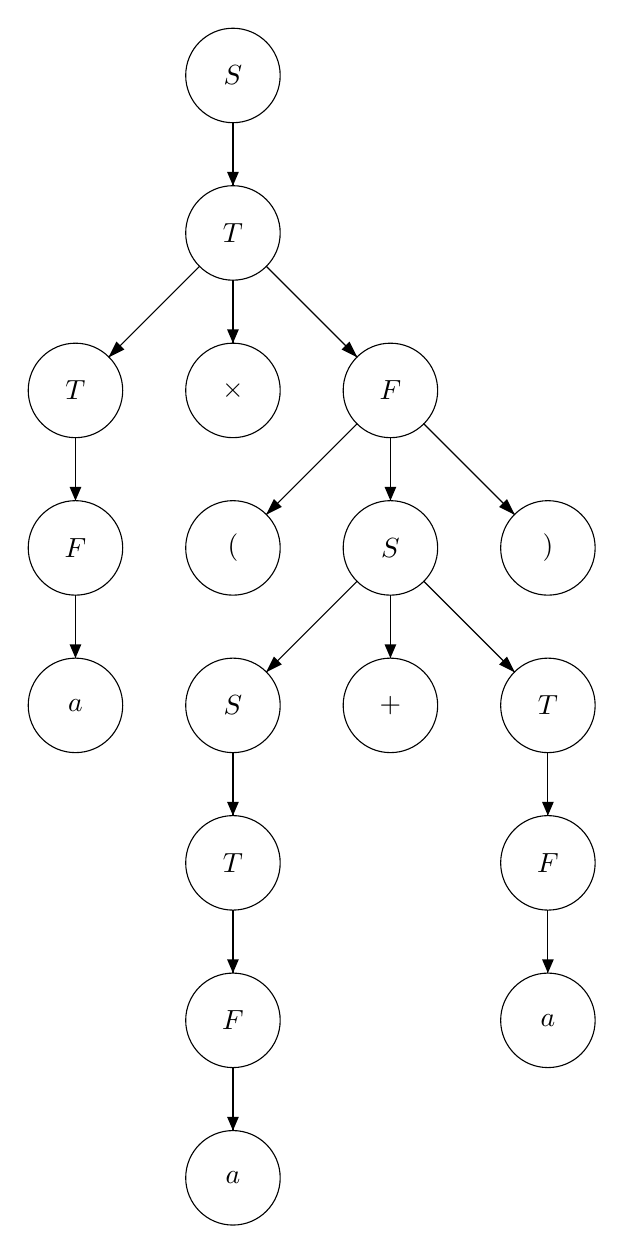
\begin{tikzpicture}[scale=0.2]
\tikzstyle{every node}+=[inner sep=0pt]
\draw [black] (0,10) circle (3);
\draw (0,10) node {$S$};

\draw [black] (0, 7) -- (0, 3);
\fill [black] (0, 3) -- (-.375, +3.875) -- (+.375, +3.875);
\draw [black] (0, 0) circle (3);
\draw (0, 0) node {$T$};

\draw [black] (-2.1, -2.1) -- (-7.9, -7.9);
\fill [black] (-7.9, -7.9) -- (-6.9, -7.4) -- (-7.4, -6.9);
\draw [black] (-10, -10) circle (3);
\draw (-10, -10) node {$T$};

\draw [black] (-10, -13) -- (-10, -17);
\fill [black] (-10, -17) -- (-10.375, -16.125) -- (-9.625, -16.125);
\draw [black] (-10, -20) circle (3);
\draw (-10, -20) node {$F$};

\draw [black] (-10, -23) -- (-10, -27);
\fill [black] (-10, -27) -- (-10.375, -26.125) -- (-9.625, -26.125);
\draw [black] (-10, -30) circle (3);
\draw (-10, -30) node {$a$};

\draw [black] (0, -3) -- (0, -7);
\fill [black] (0, -7) -- (-.375, -6.125) -- (+.375, -6.125);
\draw [black] (0, -10) circle (3);
\draw (0, -10) node {$\times$};

\draw [black] (+2.1, -2.1) -- (+7.9, -7.9);
\fill [black] (+7.9, -7.9) -- (+6.9, -7.4) -- (+7.4, -6.9);
\draw [black] (+10, -10) circle (3);
\draw (+10, -10) node {$F$};

\draw [black] (+7.9, -12.1) -- (+2.1, -17.9);
\fill [black] (+2.1, -17.9) -- (+3.1, -17.4) -- (+2.6, -16.9);
\draw [black] (0, -20) circle (3);
\draw (0, -20) node {$($};

\draw [black] (+10, -13) -- (+10, -17);
\fill [black] (+10, -17) -- (+10.375, -16.125) -- (+9.625, -16.125);
\draw [black] (+10, -20) circle (3);
\draw (+10, -20) node {$S$};

\draw [black] (+7.9, -22.1) -- (+2.1, -27.9);
\fill [black] (+2.1, -27.9) -- (+3.1, -27.4) -- (+2.6, -26.9);
\draw [black] (0, -30) circle (3);
\draw (0, -30) node {$S$};

\draw [black] (0, -33) -- (0, -37);
\fill [black] (0, -37) -- (+.375, -36.125) -- (-.375, -36.125);
\draw [black] (0, -40) circle (3);
\draw (0, -40) node {$T$};

\draw [black] (0, -43) -- (0, -47);
\fill [black] (0, -47) -- (+.375, -46.125) -- (-.375, -46.125);
\draw [black] (0, -50) circle (3);
\draw (0, -50) node {$F$};

\draw [black] (0, -53) -- (0, -57);
\fill [black] (0, -57) -- (+.375, -56.125) -- (-.375, -56.125);
\draw [black] (0, -60) circle (3);
\draw (0, -60) node {$a$};

\draw [black] (+10, -23) -- (+10, -27);
\fill [black] (+10, -27) -- (+10.375, -26.125) -- (+9.625, -26.125);
\draw [black] (+10, -30) circle (3);
\draw (+10, -30) node {$+$};

\draw [black] (+12.1, -22.1) -- (+17.9, -27.9);
\fill [black] (+17.9, -27.9) -- (+16.9, -27.4) -- (+17.4, -26.9);
\draw [black] (+20, -30) circle (3);
\draw (+20, -30) node {$T$};

\draw [black] (+20, -33) -- (+20, -37);
\fill [black] (+20, -37) -- (+20.375, -36.125) -- (+19.625, -36.125);
\draw [black] (+20, -40) circle (3);
\draw (+20, -40) node {$F$};

\draw [black] (+20, -43) -- (+20, -47);
\fill [black] (+20, -47) -- (+20.375, -46.125) -- (+19.625, -46.125);
\draw [black] (+20, -50) circle (3);
\draw (+20, -50) node {$a$};

\draw [black] (+12.1, -12.1) -- (+17.9, -17.9);
\fill [black] (+17.9, -17.9) -- (+16.9, -17.4) -- (+17.4, -16.9);
\draw [black] (+20, -20) circle (3);
\draw (+20, -20) node {$)$};
\end{tikzpicture}
\end{document}
